\documentclass[]{article}
\usepackage[english]{babel}
\usepackage{url}
\usepackage{graphicx}
\usepackage{hyperref}
\usepackage{listings}
\bibliographystyle{IEEEtranS}

% Title Page
\title{MCML with Boundary Surfaces}
\author{Marius Kircher}


\begin{document}
\maketitle

\begin{abstract}
	This project report describes an extended implementation of multi-layered Monte Carlo photon transport\cite{wang1992monte}, abbreviated as MCML. It supports structured boundaries, whereas original MCML only supported planar layers. This allows to use the accurate Monte Carlo method for simulation of light in more realistic materials. The report presents and compares radiance profiles of different boundary shapes. The focus lies on the properties reflectance and transmittance, that are important for visual appearance.
\end{abstract}

\section{Introduction}

The report will first explain the principles and purpose of Monte Carlo light transport, before moving on to related work covering MCML specifically. On this basis, the contributions made by this project are stated and explained in detail in the implementation section. The new implementation is verified against the existing work and finally results are presented.

\subsection{Monte Carlo Light Transport}

\begin{figure}[ht!]
	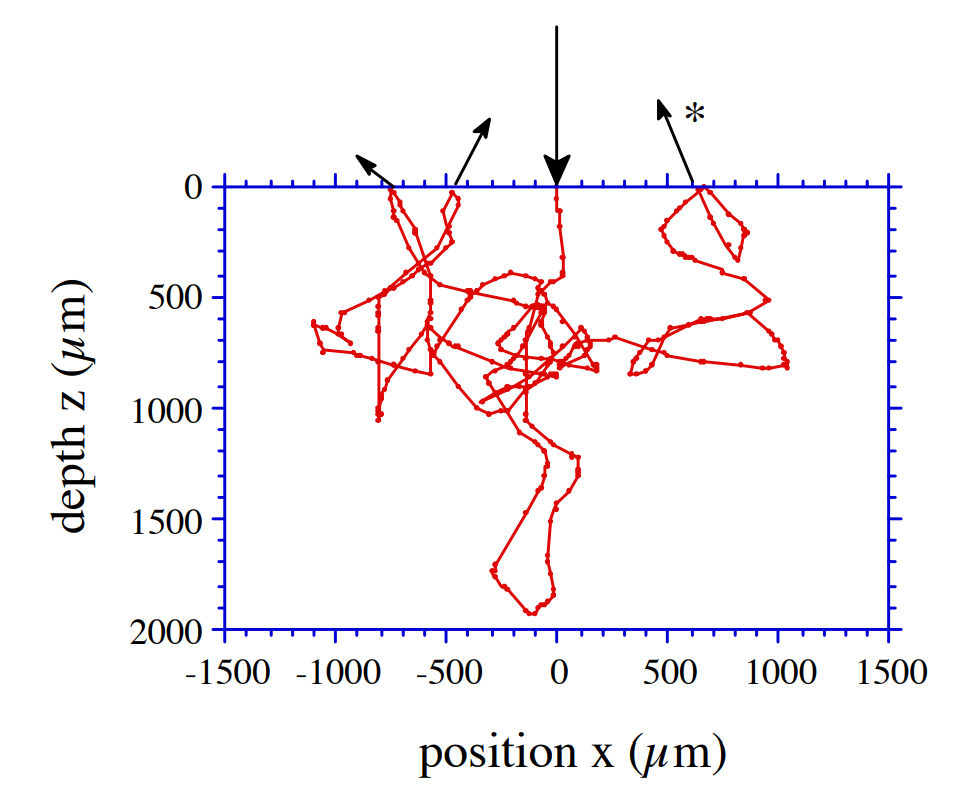
\includegraphics[width=\linewidth]{img/trajectory.png}
	\caption{A single photon walk. Taken from~\cite{wang1992monte}.}
	\label{trajectory}
\end{figure}

Monte Carlo simulation of light is very accurate, because it simulates single photon packets and records the distribution of a very large number of photons. This implies, that it is a statistical method, using a pseudo random number generator to compute, what can be thought of random walks of photons, visualized in \autoref{trajectory}.

A photon walk is defined by scattering and absorption in a specific material. These are also called the interaction properties:

\begin{description}
	\item[$\mu_s$] Scattering coefficient $[cm^{-1}]$ is the amount of scattering events per unit length
	\item[$\mu_a$] Absorption coefficient $[cm^{-1}]$ is the absorbed fraction of energy per unit length
\end{description}

In reality, these properties are also dependent on wavelength, which, in the quantum model, is equivalent to the amount of energy carried by one photon. In any case it means, that scattering and absorption are dependent on the color of the light. Since there is an infinite number of colors and natural appearance is the accumulation of subsets, computer graphics has to deal with composition from single colors. With the model used here, one can only simulate a single color at a time.

While absorption can be easily understood as energy that is transformed from light to heat, hereby leaving the considered system, scattering is more interesting. Different particles scatter light in different directions, that are generally hard to define. Simplified analytical definitions, called phase functions, are often used. They describe the angular probability distribution for photon direction changes. The popular Henyey-Greenstein phase function, that is used here, can be configured by scattering anisotropy $g$ as another material interaction property. A value of $g=0$ denotes a uniform probability distribution, i.e. isotropic scattering. Values of $g<0$ or $g>0$ control the amount of backward or forward scattering, respectively.

Finally, refractive indices are needed to compute the amounts of reflection and refraction at material boundaries according to Fresnel's formula.

\begin{figure}[ht!]
	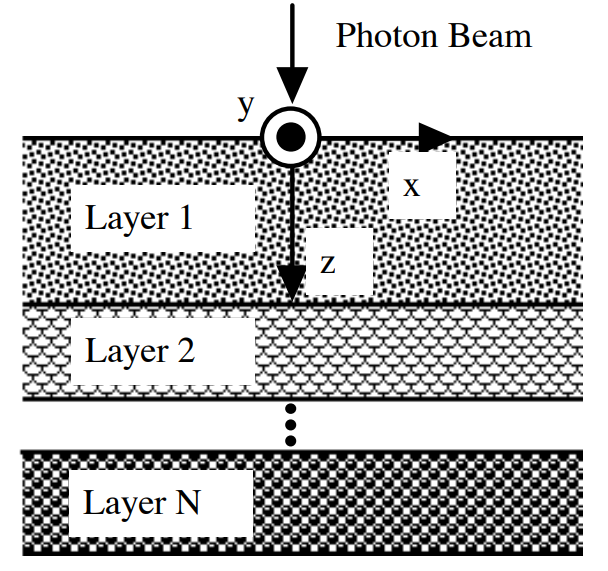
\includegraphics[width=\linewidth]{img/layer-model.png}
	\caption{MCML's layer model. Taken from~\cite{wang1992monte}.}
	\label{layer-model}
\end{figure}

The material geometry in MCML is a sequence of layers as shown in \autoref{layer-model}. Photons enter through the coordinate origin and move in 3 dimensions.

Radiance distributions are recorded only as profiles, because the material model is radially symmetric. The reflectance profile is the distribution of photons that escaped at the top layer and transmittance is the analog at the bottom layer, in other words:

\begin{description}
	\item[$R_d(r)$] Diffuse reflectance $[J/cm^2]$ as function of radius $[cm]$
	\item[$T_t(r)$] Total transmittance $[J/cm^2]$ as function of radius $[cm]$
\end{description}

There are also other recorded quantities, such as absorption, that are of less interest in this report, as they do not contribute to visual appearance.

\section{Related Work}

\subsection{Light propagation model}

\begin{figure}[ht!]
	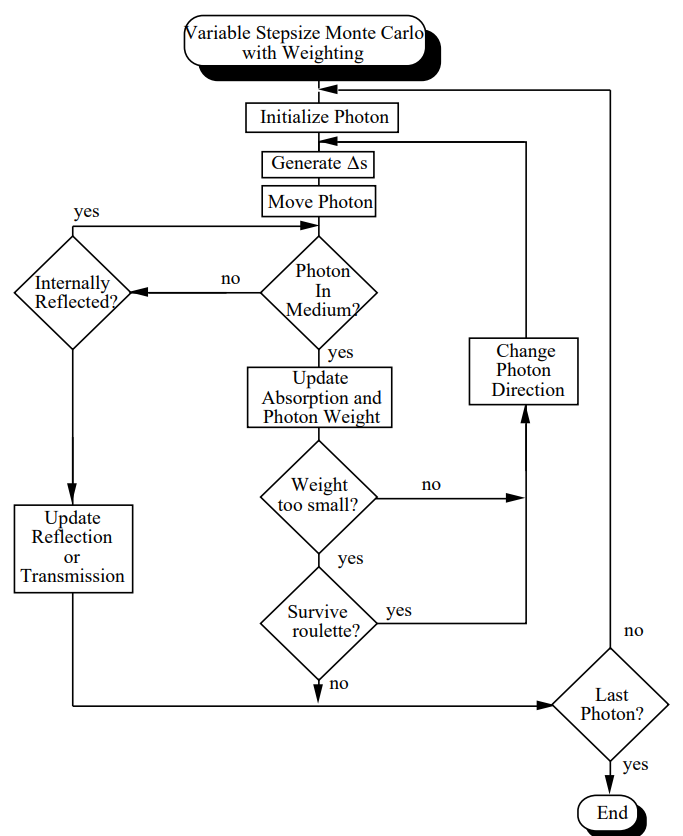
\includegraphics[width=\linewidth]{img/flowchart.png}
	\caption{Single layer Monte Carlo flowchart. Taken from~\cite{prahl89}.}
	\label{flowchart}
\end{figure}

The work is based on the light propagation model by Prahl et al.~\cite{prahl89}. You can get an overview of the algorithm by looking at the flowchart in \autoref{flowchart}.

Photons are initialized with a weight of $1.0$, which is explained in \autoref{impl:photon-transport}. Then, the photon performs a series of repeated steps. Each step length is generated by drawing a random number from a probability distribution based on the interaction coefficient $\mu_a+\mu_s$. The photon is moved by this length in the current direction. The moved photon path has to be checked for collision with the layer boundaries. After each step the photon interacts with the material.

If there was no collision, the photon drops a fraction of its weight based on $\mu_a$, which is added to total absorption. To avoid spending too much time simulating photons with small weight, i.e. small contribution to recorded quantities, but to still not bias the simulation, a so-called roulette is performed. Photons with very small weight enter the roulette. Such a photon dies with a probability $p \in (0,1)$ and if it survives, its weight is multiplied by $1/p$ as a countermeasure to the introduced bias. In the implementation described later, the weight threshold is $0.0001$ and $p=0.1$.

If the photon survives the roulette, its direction changes. A random number is drawn from the Henyey-Greenstein distribution, which yields the cosine of the deflection angle $\theta \in (0, \pi)$. This angle denotes how much the photon is diverted from its current path, i.e. is used for a rotation around an axis perpendicular to the current path. Relative to the current movement, $\theta$ can describe any change from $0$, i.e. forward scattering, to $\pi$, i.e. backward scattering. A second rotation around the axis of the current path uses a uniformly distributed angle $\psi \in (0, 2\pi)$.

If there was a collision, the algorithm decides if the photon is reflected, i.e. stays in the layer, or transmitted, i.e. leaves the medium. For this, the refraction angle is calculated using Snell's law and the refractive indices inside and outside the layer. Then Fresnel's formula is used to calculate the reflected fraction $R$. If for a uniform random number $\eta \in (0,1)$, $\eta > R$ is true, then the photon is transmitted, otherwise reflected. The algorithm (and also the implementation described later) does not perform partial reflection. If the photon leaves the layer, the remaining weight is added to the total reflection or transmission.

The simulation ends, when the target number of photons equals the number of photons, that left the layer or did not survive the roulette.

\subsection{Previous implementations}

Wang and Jacques~\cite{wang1992monte} published a C implementation of MCML in 1992 along with extensive documentation. The code is purely sequential and because of the inherently large number of photons required, it was worth working on another implementation. Alerstam et al.~\cite{alerstam2008parallel} published a GPU implementation in 2008, which uses the Nvidia CUDA interface. They achieved much faster simulations, but their program runs only on single Nvidia GPUs.

\section{Contribution}

The implementation of MCML presented here can use multiple PCs and GPUs by any vendor for parallelization and is based on OpenCL and MPI. Details are described in the implementation section.

The other contribution is support for non-planar layers. This is done by representing boundaries as radially symmetric heightfields, where the symmetry allows to store only a 1-dimensional array of height samples. Non-symmetric heightfields would only make sense, once photon distributions are also recorded in two dimensions. Additionally, each height value is associated with a spacing, to enable irregular grids. The surface between height samples is defined by linear interpolation. In 3-dimensional space, a surface is therefore a sequence of connected concentric capped cones of finite height.

\section{Implementation}

\subsection{Parallelization}

Simulating individual photon packets is well suited for parallelization. The implementation does this on two levels.

On the first level, work is distributed onto multiple PCs that are connected by a local network. For this use case exists the Message Passing Interface (MPI), which provides a standardized C API and is based on inter-process communication. Before running MPI programs, one has to make sure, that if authentication is in place, all PCs can be accessed with the same username and password. Then the MPI listener service can be started on each node. The own program executable is passed to the MPI execution program, which connects to the listeners and starts a process on each node. MPI allows to query the number of nodes and the current node identifier, also called rank, from within the program. In general, all nodes use the same code for processing, but for I/O one node executes a special branch. It reads the input file and synchronizes data with an MPI Broadcast. All nodes work on the simulation and call the MPI Reduce function to compute the total sum of the resulting radiance arrays. Note that Reduce has to wait for all nodes to finish simulation. Finally, the I/O node writes the radiance data to the output file.

On the second level, work is further split on GPU threads. We chose OpenCL for this task, since it is available for all relevant GPU architectures. An OpenCL kernel implements the actual MCML photon transport for one photon packet. The maximum number of threads can be queried through OpenCL and depends on used registers and other GPU hardware resources. The kernel computes a fixed number of bounces to limit the time spent on the GPU, because the operating system would kill a process that blocks the GPU for too long. The program maintains an array by which it assigns one photon packet to one thread and repeatedly starts GPU runs, followed by checking the array for photon packets to be restarted until the target amount has been reached.

Work distribution is possible using different strategies. One implemented approach assumes equal processing power among MPI nodes and divides the total target number of photons up-front by the number of nodes, before each node starts its part of the simulation (note that we use the term photon, when we actually refer to photon packets, which is explained in \autoref{impl:photon-transport} about photon transport). In practice, this approach did not work well. Specifically, it sometimes caused MPI to abort because of a timeout during Reduce. Therefore a more fine-grained prallelization approach was implemented as follows.

First, we divide MPI nodes in several workers and one master. We can run a batch of $N$ photons in parallel, where $N$ equals thread count. In order to limit time spent on GPU, we always run for a fixed number of bounces. We cannot know how many runs it will take until the batch is finished (all photons terminated). Instead we count finished photons after each run. If after run $i$, a number $K > Z$ photons have finished, the worker sends $K$ to master. One thread of the master must be in receiving state. If the master finds that the number of photons that is not being worked on is $L >= K$, the response is CONTINUE, otherwise FINISH. When receiving CONTINUE, the worker spawns $K$ new photons, otherwise it finishes the remaining photons (with thread utilitization $< N$) and calls Reduce on its output arrays. When $L$ drops to zero, the master also calls Reduce, collects the total result and writes it to file.

After the master responds with FINISH, he finishes the remaining $L$ photons on his own, because there is no guarantee that a worker has space for exactly $L$ photons at some point, meaning (in the negative case) they could either run too many or $L$ never drops to zero.

With this approach, Reduce did not cause timeouts, since all workers receive a FINISH response within a short amount of time, because of the high communication frequency.

The high communication frequency, on the other hand, leads to a trade-off between thread utilization and communication efficiency, both impacting performance to yet unknown extent. If we set $Z$ to zero, we get maximum thread utilization, but high communication overhead. The higher $Z$ becomes, the worse thread utilization and the better communication efficiency becomes.

\subsection{MCML Kernel}
\label{impl:photon-transport}

The MCML kernel performs the actual photon transport. As input it receives an array of layers, where each layer contains interaction properties of its material, and an array of boundaries containing the geometry information. In contrast to existing MCML implementations, it seemed reasonable to split these two classes of information, because supporting different boundary surfaces requires more involved geometric data and operations.

The output consists of three radiance arrays for diffuse reflectance, absorbance and transmittance. The arrays can be thought of histograms over radius with $n_r$ bins of size $d_r$ centimeters, respectively. A second dimension can be added by specifying a number of depth bins $n_z > 1$ of size $d_z$ for the absorption array, or a number of angular bins $n_a > 1$ for the reflectance and transmittance arrays. See the MCI file format in~\cite{wang1992monte}.

A photon packet is defined as having an energy weight of $1.0$ when it is launched. The weight may be reduced multiple times by absorption during the walk, before the remaining fraction is added to a total radiance, which is finally normalized by the number of photon packets simulated. This reduces variance, compared to a simulation of photons, that really behave atomically. The packet, however, behaves like a single photon in the sense that it has a single path.

An additional data structure is the array of photon states, which is needed to preserve state across GPU runs. A photon state contains current position, direction, layer index, weight and state of the xorshift~\cite{marsaglia2003xorshift} random number generator. When a state is initialized, a hash function is used on the state index to seed the xorshift generator.

\subsection{Boundary Specification}

Previous MCML implementations used flat boundaries, that were implicitly defined by the layers. The implementation presented here supports both implicit boundaries and explicitly defined heightfields.

Heights are interpreted from heightfield origin, which is defined by layer thicknesses, into negative z-direction, because in MCML the z-axis points \emph{down} into the material. The last height sample is valid for all radii that are out of bounds.

To enable mixing implicit and explicit boundaries in the same simulation, the MCI file format was extended. Lines containing explicit boundary data start with 'b', then the number of samples and then the list of sample values, which consists of alternating heights and spacings. This is an excerpt from an example MCI file:

\begin{lstlisting}
[...]

2 # Number of layers
1 # n for medium above

# explicit heightfield boundary with 2 samples
b 2 0.2.1 0.0 0.1

# n mua mus g d
1.4 0.1 90  0 0.5 # layer 1

# implicit flat boundary

1.4 0.1 90  0 0.5 # layer 2

# explicit heightfield boundary with 3 samples
b 3 0.2 0.1 0.1 0.1 0.0 0.1

1 # n for medium below
\end{lstlisting}

Old formats are supported by the new implementation.

Explicit heightfield boundaries can also be turned on or off globally for performance reasons. When the kernel define IGNORE\_HEIGHTFIELDS is set, any explicit boundary data from the file is ignored.

The recorded radiance is clamped, so that all photon packets that fall outside the array bounds are accumulated at the edges. In original MCML this could only happen in xy directions. Now also the depth index of the absorption detection array must be clamped, as we can have for example weight drops at a depth less than zero.

The implementation checks if heightfields overlap each other before starting the simulation. Overlapping heightfields constitute an invalid layer model.

\subsection{Boundary Intersection}

After each step of a photon packet, the moved line has to be tested for an intersection with two radial heightfields, the one at the top of the current layer and the one at the bottom.

The base of the heightfield intersection algorithm is an analytical method for intersecting rays with cones by David Eberly\cite{schneider2002geometric}. The cone shapes arise when the radial 1D heightfield is rotated in the xy-plane around the origin. The algorithm is outlined in the following.

First we must find all potential cones in the path of the line. We assign an ascending index from inner to outer cones. To find the highest candidate index, we count the spacings, that fit into the length of the xy-vectors of the start and end of the line, and take the maximum. The lowest candidate index is obtained by projecting the heightfield origin onto the line and count the spacings that fit into the length of the xy-vector of the resulting point. All cones between these two indices, inclusively, are tested for intersection with the line and the closest hit is returned.

To calculate reflections and transmissions at heightfield boundaries, a normal is needed. The line-cone intersection method was extended to additionally return the normal at the point of intersection. There are sharp local minima and maxima where the gradient cannot be defined, since the heightfield is interpolated linearly. For these cases the boundary is treated as a xy-plane with normal along z-axis. The direction of the normal is always chosen to point into the half space from where an intersecting ray comes in.

If there was an intersection in the last photon step and the photon is still inside the simulation domain, the corresponding boundary has to be temporarily disabled for intersections during the next step. The reason for this is that the photon might not be moved exactly onto the boundary surface, because of limited floating point accuracy, and it would therefore be possible to detect another erroneous intersection with the same boundary.

There is a fallback to a faster intersection test with a plane, if a boundary is not a heightfield.

\subsection{Building and Running}

When building the program for the first time on a new computer, you have to set the paths to your compiler, OpenCL and MPI libraries in the Makefile. Then use nmake to build. For execution, use the following command:

\begin{lstlisting}
mpiexec /machinefile mpi.txt /pwd "***"
clustermcml-windows.exe mcmlKernel.c "-Werror" sample.mci
\end{lstlisting}

where the machinefile mpi.txt specifies the IP address and number of processes per MPI node. The executable is called clustermcml-windows and receives as first argument the MCML kernel file, which will be compiled by the OpenCL implementation. After the kernel file follow the OpenCL compiler arguments, where this example wants to print all warnings as errors. On the tested machines, the current kernel code did not generate warnings. You can add other compiler flags, such as "-D IGNORE\_A" to skip writing to absorption array or "-D IGNORE\_HEIGHTFIELDS" to use implicit flat boundaries, where both options exist to speed up simulation times.

The implementation was currently only built and run on Microsoft Windows, but all used libraries are also available on other platforms. There is no build system other than make (on Windows: nmake) in place, because the project is relatively small and simple. The Makefile can be altered with analog compiler commands and flags, as well as runtime and library paths.

\subsection{Limitations}

To obtain a height value at arbitrary floating point coordinates, the heightfield must be interpolated. Therefore it would make sense to store them in textures and use built-in access operators on the GPU. Currently, the program uses raw buffers and does interpolation in code.

\section{Verification}

\section{Results}

\section{Conclusion}

\bibliography{bibliography}
\end{document}          
